% !TEX program = xelatex
\documentclass[10pt,letterpaper,twocolumn]{article}

% === GEOMETRY ===
\usepackage[top=0.75in, bottom=0.75in, left=0.75in, right=0.75in]{geometry}

% === FONTS ===
\usepackage{fontspec}
\usepackage{unicode-math}
\setmainfont{Latin Modern Roman}[
  Extension=.otf,
  UprightFont=lmroman10-regular,
  BoldFont=lmroman10-bold,
  ItalicFont=lmroman10-italic,
  BoldItalicFont=lmroman10-bolditalic,
]
\setsansfont{Latin Modern Sans}[
  Extension=.otf,
  UprightFont=lmsans10-regular,
  BoldFont=lmsans10-bold,
  ItalicFont=lmsans10-oblique,
  BoldItalicFont=lmsans10-boldoblique,
]
\setmonofont{Latin Modern Mono}[
  Extension=.otf,
  UprightFont=lmmono10-regular,
  ItalicFont=lmmono10-italic,
  Scale=0.85,
]
\newfontfamily\acbold{ywft-processing-bold}[
  Path=../../system/public/type/webfonts/,
  Extension=.ttf
]
\newfontfamily\aclight{ywft-processing-light}[
  Path=../../system/public/type/webfonts/,
  Extension=.ttf
]

% === PACKAGES ===
\usepackage{xcolor}
\usepackage{titlesec}
\usepackage{enumitem}
\usepackage{booktabs}
\usepackage{tabularx}
\usepackage{fancyhdr}
\usepackage{hyperref}
\usepackage{xurl}
\usepackage{graphicx}
\usepackage{ragged2e}
\usepackage{microtype}
\usepackage{natbib}

% === COLORS ===
\definecolor{acpink}{RGB}{180,72,135}
\definecolor{acpurple}{RGB}{120,80,180}
\definecolor{acdark}{RGB}{64,56,74}
\definecolor{acgray}{RGB}{119,119,119}
\definecolor{acgreen}{RGB}{70,200,90}
\definecolor{draftcolor}{RGB}{180,72,135}

% Draft status is carried by the running header and the title-page notice
% below — no diagonal watermark (it interfered with two-column vertical
% spacing, stretching short columns; keymaps carries none either).

% === HYPERREF ===
\hypersetup{
  colorlinks=true,
  linkcolor=acpurple,
  urlcolor=acpurple,
  citecolor=acpurple,
  pdfauthor={@jeffrey},
  pdftitle={Gaps in Granularity: Expressive Control and the Impoverishment of Consumer Playback},
}

% === SECTION FORMATTING ===
\titleformat{\section}
  {\normalfont\bfseries\normalsize\uppercase}
  {\thesection.}
  {0.5em}
  {}
\titlespacing{\section}{0pt}{1.2em}{0.3em}

\titleformat{\subsection}
  {\normalfont\bfseries\small}
  {\thesubsection}
  {0.5em}
  {}
\titlespacing{\subsection}{0pt}{0.8em}{0.2em}

% === HEADER/FOOTER ===
\pagestyle{fancy}
\fancyhf{}
\renewcommand{\headrulewidth}{0pt}
\fancyhead[C]{\footnotesize\color{draftcolor}\textit{Working Draft --- not for citation}}
\fancyfoot[C]{\footnotesize\thepage}

% === LIST SETTINGS ===
\setlist[itemize]{nosep, leftmargin=1.2em, itemsep=0.1em}
\setlist[enumerate]{nosep, leftmargin=1.2em}

% === COLUMN SEPARATION ===
\setlength{\columnsep}{1.8em}

% === PARAGRAPH SETTINGS ===
\setlength{\parindent}{1em}
\setlength{\parskip}{0.3em}

% Hyphenation for narrow two-column layout
\tolerance=800
\emergencystretch=1em
\hyphenpenalty=50

% Two-column pages with figures often leave a column slightly short; let the
% bottom go ragged instead of stretching interline/inter-paragraph glue (which
% otherwise spreads a paragraph's own lines apart). Keep float separation
% rigid so the space around figures does not inflate either.
\raggedbottom
\setlength{\textfloatsep}{16pt}
\setlength{\floatsep}{14pt}
\setlength{\intextsep}{14pt}


\newcommand{\acdot}{{\color{acpink}.}}
\newcommand{\ac}{\textsc{Aesthetic.Computer}}

% Version / history stamps — written by cli.mjs's xelatex build (git hash +
% revision). Force the local ./ path so we never pick up a distribution
% version.tex; dev fallback so the paper still compiles standalone.
\IfFileExists{./version.tex}{\input{./version.tex}}{\providecommand{\paperhash}{dev}\providecommand{\paperrev}{0}}
\IfFileExists{./history.tex}{\input{./history.tex}}{\providecommand{\paperhistory}{}}

\begin{document}

\twocolumn[{%
\begin{center}
{\acbold\fontsize{24pt}{28pt}\selectfont\color{acdark} gaps in {\color{acgreen}granularity}{\color{acpink}.}}\par
\vspace{0.25em}

\includegraphics[width=0.6\textwidth]{figures/cover}\par
\vspace{0.15em}
{\aclight\fontsize{11pt}{13pt}\selectfont\color{acpink} Expressive Control and the Impoverishment of Consumer Playback}\par
\vspace{0.6em}
{\normalsize\href{https://prompt.ac/@jeffrey}{@jeffrey}}\par
{\small\color{acgray} Aesthetic{\acdot}Computer}\par
{\small\color{acgray} ORCID: \href{https://orcid.org/0009-0007-4460-4913}{0009-0007-4460-4913}}\par
\vspace{0.3em}
{\small\color{acpurple} \url{https://aesthetic.computer}}\par
\vspace{0.6em}
{\color{acpink}\rule{\textwidth}{1.5pt}}
\vspace{0.5em}
\end{center}

\begin{center}
{\small\color{draftcolor}\textbf{[ working draft --- not for citation ]}}
\end{center}
\vspace{0.3em}

\begin{quote}
\small\noindent\textbf{Abstract.}
A DJ dragging a record under a needle controls playback with a bandwidth the apps you actually listen and watch through will not give you. The scratch is continuous, gestural, pitch-and-time coupled, and its feedback is the sound itself, arriving in under ten milliseconds. Set that against how the platforms that own listening and watching --- YouTube, Spotify, Netflix, Apple, Instagram --- let you touch a recording: a dropdown of round numbers. \emph{0.5$\times$, 1$\times$, 1.25$\times$, 1.5$\times$, 2$\times$.} Some offer nothing at all; Spotify still plays every music track at exactly one speed and refuses to let you change it. This paper names the gap between those two worlds \emph{granularity}, and argues it is not a niche complaint but a large opening left where it matters most --- the default transport of the surfaces that own consumer listening and watching. I ground the argument in the theory of directness~\citep{hutchins1985direct}, in Buxton's account of continuous degrees of freedom and input bandwidth~\citep{buxton2007multitouch}, and in the mature craft of turntablism~\citep{hansen2010scratching} and elastic audio~\citep{ableton2024warp}, which prove that fine, expressive, real-time control of recorded sound is a solved problem the consumer layer simply declines to expose. Then I show that \ac{}~\citep{scudder2026ac} already ships this control across its players by default --- pieces where scrubbing, speed, and pitch are continuous gestures with the output as their feedback --- and argue that the itemized speed menu is a temporary artifact of an industry that mistook playback for a settings panel instead of an instrument.
\end{quote}
\vspace{0.5em}
}]

% \twocolumn[...] (the title block) resets to \flushbottom; re-assert ragged
% bottoms here so short columns beside a figure don't get their lines stretched.
\raggedbottom

\section{Introduction}

Put a finger on a spinning record and you have just done something no streaming app will let you do. You have grabbed the audio. Push and it speeds up and rises in pitch; pull back and it drops and reverses; hold and it stops dead; nudge and the whole track lurches a few milliseconds against the beat. The control is continuous --- every position of your hand maps to a position in the sound. It is gestural --- the instrument is your arm, not a button. And it is closed-loop --- the feedback is the sound itself, not a number on a readout, arriving fast enough that your ear cannot tell the touch and the tone apart. This is forty-year-old technology. A teenager with a used turntable has more expressive authority over a recording than a Spotify Premium subscriber has over anything in the catalog.

Now open YouTube and try to move through a video the way the DJ moves through a groove. You cannot. You get a dropdown. \emph{Normal. 1.25. 1.5. 1.75. 2.} A short list of round multipliers, applied globally, with no gestural surface, no pitch you can bend, no way to lean into a passage and back off --- and, until recently, no feedback at all except the changed pace once you let go of the menu. Spotify is worse: for music, the number of speeds you are offered is one. The most valuable listening surface ever built treats the play rate of a song as a constant of nature.

I call the distance between these two worlds a \emph{gap in granularity} (Figure~\ref{fig:gap}). On one side, playback is an instrument --- continuous, gestural, felt. On the other, it is a settings panel --- a finite menu of discrete states you pick from and wait on. The gap is not small and it is not cosmetic. It is the difference between \emph{performing} a recording and \emph{configuring} one.

\begin{figure}[t]
\centering
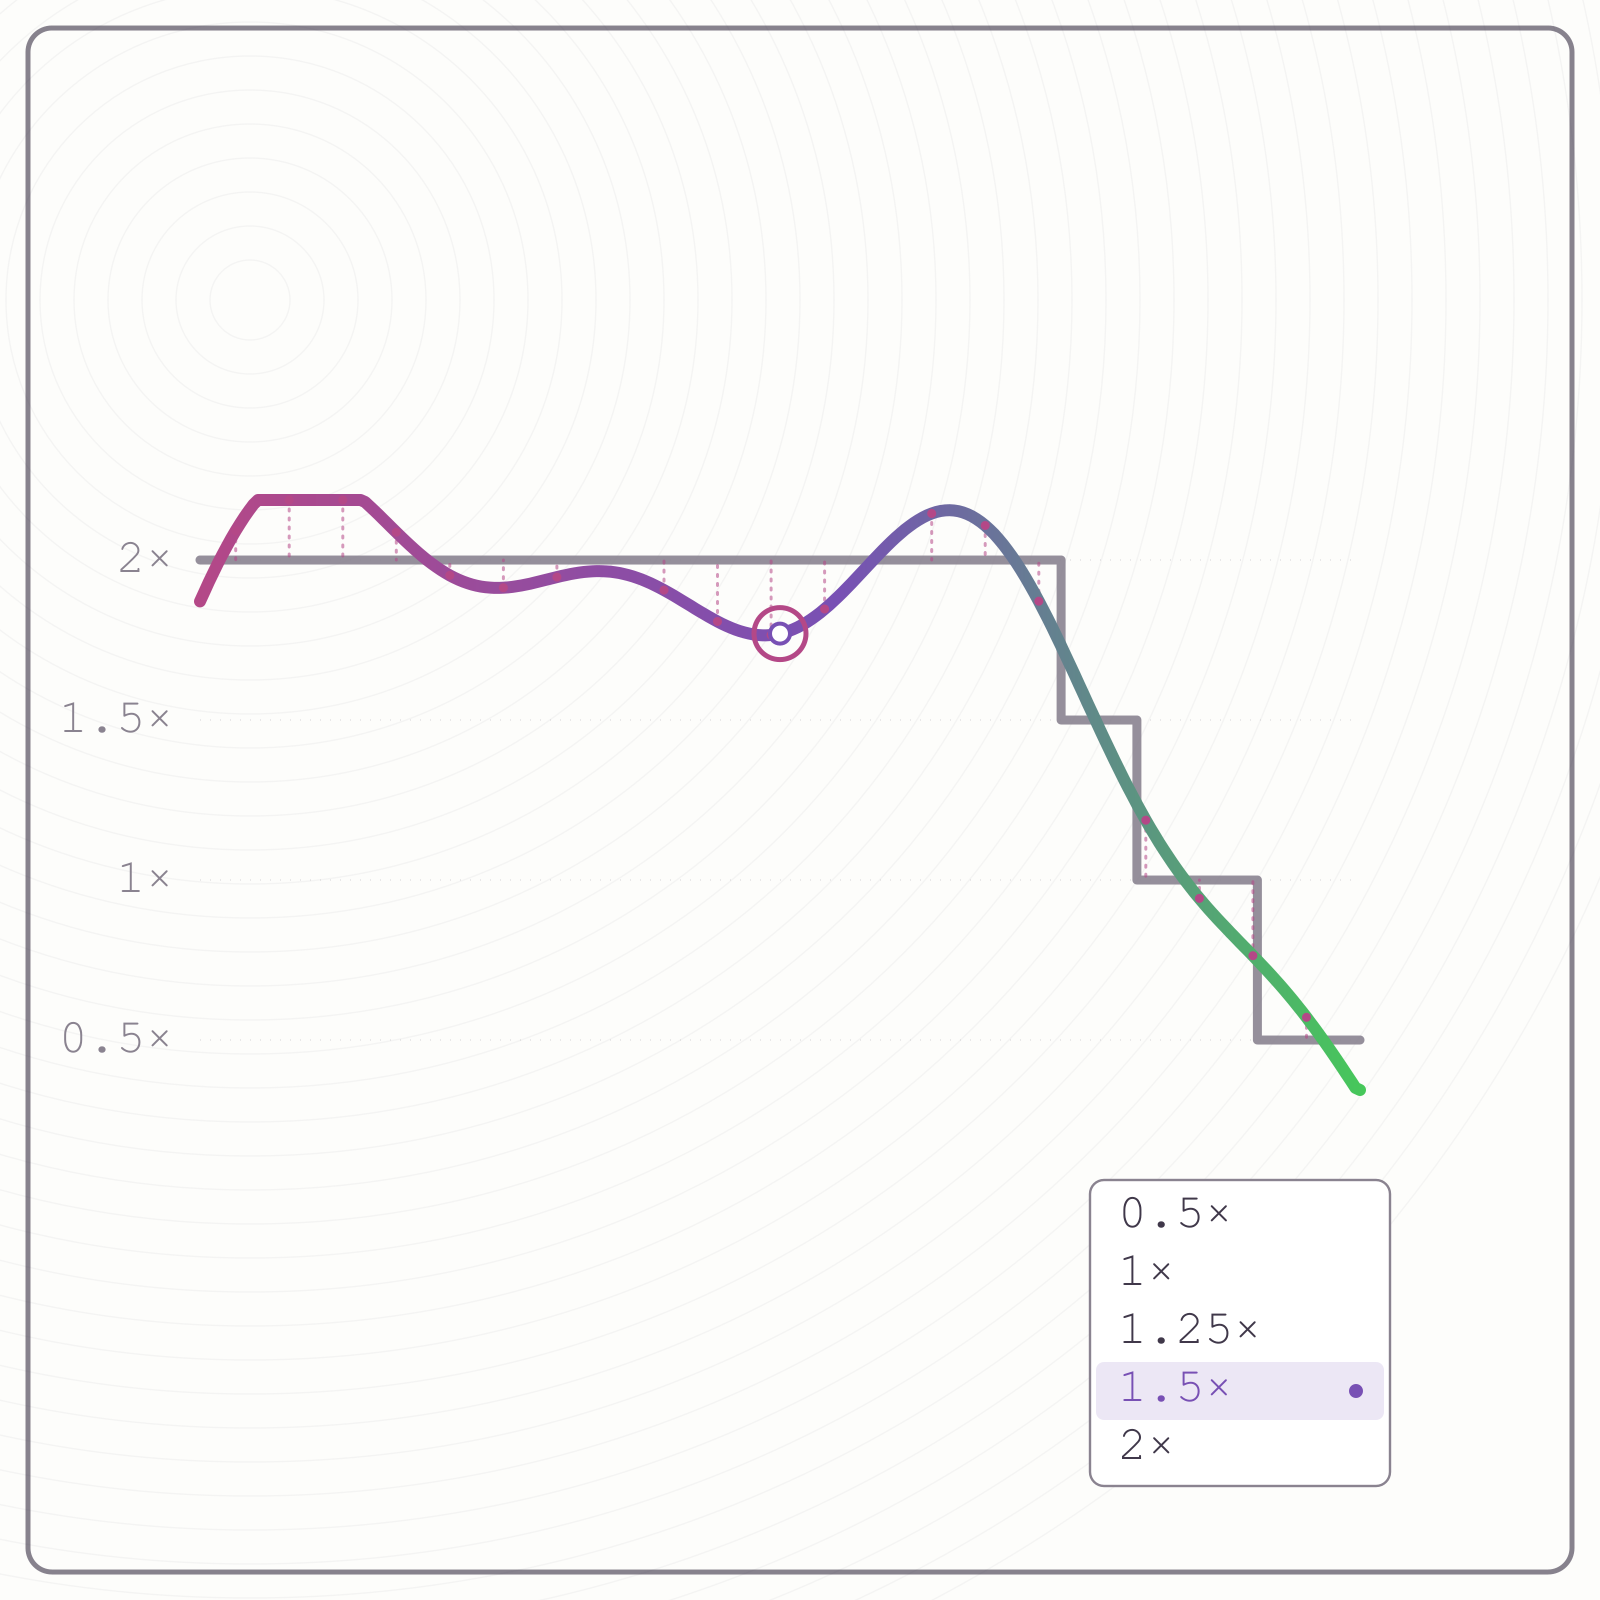
\includegraphics[width=\columnwidth]{figures/granularity-gap-diagram}
\caption{The gap, drawn. The smooth gradient curve is an expressive playback gesture --- a hand's continuous demand on the play rate, wandering freely between $0.5\times$ and past $2\times$. The grey staircase is what a speed menu makes of it: the same intention snapped to the nearest of four presets ($0.5\times$, $1\times$, $1.5\times$, $2\times$). The dashed pink connectors measure the error between them at each instant --- that error \emph{is} the granularity gap. The white-cored ring rides the gesture like a needle in a groove; the dropdown, lower right, is the impoverished control the paper indicts.}
\label{fig:gap}
\end{figure}

The argument of this paper is threefold. First, that the itemized speed menu is a genuine design failure with a precise diagnosis in HCI's oldest literature, not a reasonable simplification. Second, that expressive, fine-grained, real-time control of recorded media is a fully solved craft --- turntablists and audio engineers have practiced it for decades and the algorithms are mature and cheap --- so the consumer layer's coarseness is a choice, not a limit. Third, that \ac{} already ships the alternative: players where speed, position, and pitch are continuous gestures with the sound and image as their own feedback, on by default, on a phone. That last part is why this is not just criticism. There is a large consumer gap here, it is unclaimed, and one of the ways to see it clearly is to look at a system that already closed it.

\section{The Theory of Directness}

The vocabulary for what is wrong with the speed dropdown was written in 1985. \citet{hutchins1985direct}, in \emph{Direct Manipulation Interfaces}, argued that the feeling of directly manipulating an object arises from two things: short \emph{distance} between your intention and the action the system offers, and \emph{engagement}, the sense that you are acting on the object itself rather than describing an action to an intermediary. They split distance into two kinds. \emph{Semantic} distance is how far the system's concepts sit from the ones in your head. \emph{Articulatory} distance is how far the physical form of your action --- what your hand actually does --- sits from the meaning of that action.

The speed dropdown is a machine for maximizing articulatory distance. What you want is a rate --- a smooth, one-dimensional quantity, the same kind of quantity your hand produces when it moves faster or slower. What the interface gives you is a symbolic act: open a menu, read a list of tokens, choose the token \texttt{1.5$\times$}, dismiss the menu. You are not moving the rate. You are naming one of five rates from a controlled vocabulary. \citet{norman1988everyday} would call the space between "I want it a little faster" and "select the fourth item" a \emph{gulf of execution} --- and the dropdown makes you cross it symbolically every time, with a controller (a discrete list) whose form has nothing in common with the continuous thing it sets.

Engagement is the second casualty. \citet{shneiderman1983direct}, who coined \emph{direct manipulation}, built it on a \emph{continuous representation of the object of interest}, acted on by \emph{physical actions} rather than command syntax, through \emph{rapid, incremental, reversible} operations whose effect is immediately visible. Dragging a record satisfies every clause: the object is continuously present under your hand, the action is incremental and reversible in the same gesture, and the effect --- the sound --- is immediate. A speed menu satisfies none. The object of interest disappears behind a chrome popover; the action is a discrete jump; reversal means reopening the menu; and the effect is deferred until after you commit.

There is a hard number under "immediate." \citet{nielsen1993usability} fixes 0.1 seconds as the threshold below which a response feels instantaneous --- the point at which the user perceives the system as reacting rather than replying. Direct manipulation lives entirely inside that window; you drag and the world moves with your hand. And the tolerance is not folklore --- it is measured: \citet{annett2014low} find that for continuous inking, the lag between the pen and the mark it leaves becomes perceptible in the low tens of milliseconds, an order below Nielsen's already-tight bound. The turntablist's standard is stricter still. Scratching is built from percussive gestures timed to the tens of milliseconds --- the crossfader cut several times a second, pitch events on the order of tens of ms~\citep{hansen2010scratching}. Latency on that same scale, sitting between the hand and the sound, would smear the very attack the technique is made of; the demand for tight, low-latency, closed-loop coupling between gesture and result is what \citet{wessel2002intimate} name \emph{control intimacy}. \citet{omodhrain2000playing} shows that loop is not only auditory but haptic --- the instrument pushing back against the hand is itself part of the control. The speed dropdown does not even try to enter that budget.

The last piece is Buxton's. The richness of an interaction, he argues, tracks the number of \emph{continuous degrees of freedom} the input affords~\citep{buxton2007multitouch,buxton2018gesture}. A menu selection is zero continuous degrees of freedom --- a choice among labels. A slider is one, sampled coarsely. A finger dragging across a groove is a continuous position \emph{and} a velocity \emph{and}, on a good surface, pressure --- several coupled dimensions streaming at the frame rate of the hand. \citet{buxton1986chunking} calls the difference \emph{chunking}: a good gesture lets you perform an entire phrase --- speed up here, hold, snap back --- as one motor act, where the menu forces you to decompose the same intention into a sequence of discrete selections. HCI has a name for the axis, too. Card, Mackinlay and Robertson's design space of input devices treats a control's \emph{resolution} --- its granularity --- as a first-class property, and a playback rate is natively a continuous, high-resolution dimension that the menu resamples down to four points~\citep{card1991morphological}. Buxton had put it more bluntly still: conventional interfaces throw away most of the hand's continuous motor bandwidth before the user ever gets to spend it~\citep{buxton1986more}. Consumer playback UIs have spent fifteen years converging on the zero-degree end of that scale.

\section{The Coarse Menu, Itemized}

It is worth being specific about how little the dominant platforms actually give you, because the poverty is easy to miss when you have never been offered anything better.

\textbf{YouTube} offers discrete presets from 0.25$\times$ to 2$\times$, and, more recently, a "custom" slider that moves in 0.05 steps within that range (Figure~\ref{fig:youtube})~\citep{youtube2026speed}. This is the generous end of the consumer spectrum, and it is still a global multiplier with no gestural surface, no pitch control, and no coupling to the content: you set a number and the whole video obeys it. Scrubbing the timeline is separate from setting the speed, and neither one is expressive --- the scrub bar is a seek, not a performance.

\begin{figure}[t]
\centering
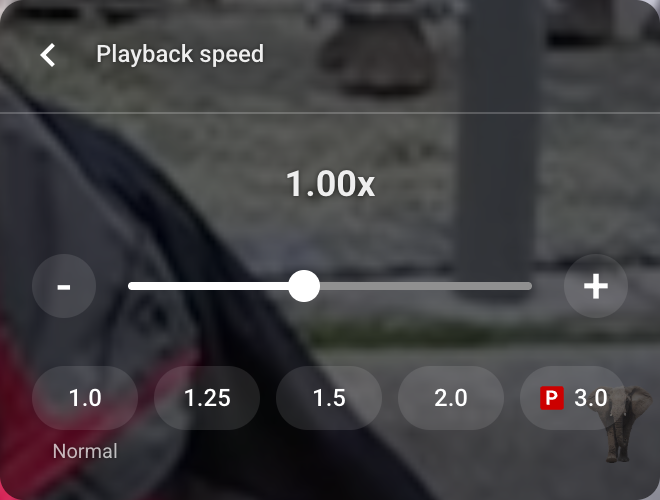
\includegraphics[width=\columnwidth]{figures/fig-youtube-speed}
\caption{YouTube's playback-speed control, 2026 --- the generous end of the consumer spectrum. A slider that snaps to a row of presets ($1{\times}$ ``Normal'', $1.25$, $1.5$, $2$, and a Premium-gated $3.0$), applied globally to the whole video. There is no coupling to the content, no pitch to bend, and nothing continuous under the finger. The ``instrument'' is a list of numbers you pick from and release.}
\label{fig:youtube}
\end{figure}

\textbf{Spotify} is the instructive case. For music --- the core of the product --- there is no speed control at all. Every track plays at 1.0$\times$, always, and years of it sitting among the most-requested items in the community forums have not changed it~\citep{spotify2026speed}. Speed adjustment exists only for podcasts and audiobooks, as a small set of increments from 0.5$\times$ to 3$\times$. The company that convinced the world to rent its music instead of owning it has decided that the one thing you may not do to a song is change how fast it moves.

\textbf{Audible} is the quiet best-in-class: 0.5$\times$ to 3.5$\times$ in 0.1 increments --- thirty-one discrete speeds~\citep{audible2026speed}. Notably, the platform that treats speed most seriously is the one whose content is pure information --- spoken words, where faster is simply more words per minute and the "instrument" framing never comes up. Granularity, on the consumer side, has been allowed to exist only where expression is beside the point.

\textbf{Netflix} gives five presets; \textbf{Apple Music} gives nothing; \textbf{TikTok} and \textbf{Instagram} give a small preset set plus a press-and-hold that jumps to a single fixed 2$\times$ and back. \textbf{Apple Podcasts} is the one that has quietly moved: since iOS~26 it offers a 0.5--3$\times$ slider in 0.1 steps, finer than most --- and still a discrete, global setting. That press-and-hold deserves naming, because it is the closest the platforms come to a gesture, and it makes the point better than its absence would. It is real, it is a gesture, and it is a \emph{binary trigger of one preset} --- zero continuous degrees of freedom, no way to lean into a passage and back off. A gesture wired to a menu is still a menu.

It is the same impoverishment \citet{moore1988dysfunctions} diagnosed in MIDI: quantize a continuous performance gesture into a coarse grid of discrete values and you throw away the very bandwidth that carried the expression. The itemized speed control is the MIDI-fication of playback rate. Across every one of these surfaces the pattern holds --- playback rate is modeled as a \emph{setting} you configure, not a \emph{parameter of performance} you hold in your hand. None offers \emph{continuous, content-coupled control of the play rate}. None gives real-time closed-loop feedback as you adjust it. None lets you couple or decouple pitch and time by hand, or touch a single moment and stretch it. The default transport of the platforms that own passive listening and watching has standardized on the least expressive control surface HCI can describe.

One clarification pre-empts the obvious objection. Apple's players \emph{do} offer a continuous, gestural scrub: touch-hold the scrubber and drag to move between Hi-Speed, Half-Speed, and Fine, with haptic detents~\citep{apple2026scrubbing}. But that gesture controls \emph{seek precision} --- how fast the playhead travels while you drag it --- not the \emph{rate of play}. The playhead moves under your finger; the speed the recording plays at, the moment you let go, is still a menu. Seek is not the instrument. Rate is.

\section{The Expressive Ceiling We Already Cleared}

The coarseness would be forgivable if fine, real-time control of recorded audio were hard, exotic, or unsolved. It is none of those things. It is a mature craft with a research literature, a professional practice, and cheap, shipping algorithms.

Turntablism is the existence proof at the human end. \citet{hansen2010scratching}, in a full doctoral thesis on the acoustics and performance of scratching, treats the DJ's hand as a high-resolution musical controller and models the mapping from gesture to sound in detail. \citet{hansen2006mapping} lay out the parameter mappings --- position to playback phase, velocity to pitch and rate, the crossfader as an amplitude gate --- that let a performer improvise emotion into a record in real time. The technique has been formalized enough to build instruments around: the \emph{Skipproof} virtual turntable lets non-experts execute complex scratch gestures through simplified high-level controls~\citep{hansen2010skipproof}, and Lopes explores alternative multitouch interfaces for DJing on a phone~\citep{lopes2010mtdjing}. Its cultural history is documented in as much depth as its acoustics: \citet{katz2012groove} traces scratching from a mid-1970s Bronx accident into a codified, competitive, globally taught art form, and \citet{farrugia2012beyond} and \citet{rodgers2010pink} follow the same instruments --- vinyl, mp3, DJ and synthesis software --- into the question of who is invited to command them, and who has been written out of the story. And designing the expressive gesture-to-sound mappings underneath it is a live research practice of its own~\citep{fiebrink2009meta}; performing on newly-built musical interfaces is by now a live art in itself~\citep{knotts2015algorithmic}. This is not folk knowledge. It is a studied, teachable, decades-deep discipline of expressive playback --- and its entire premise is the continuous, gestural, low-latency control that consumer apps refuse.

Elastic audio is the existence proof at the tool end. Every serious production environment already treats a recording as a stretchable material. Ableton Live's Warp modes use granular resynthesis to decouple time from pitch, so you can slow a passage without dropping its key or drag its tempo around a grid in real time~\citep{ableton2024warp}. Pro Tools' Elastic Audio does real-time time-stretch and pitch-shift on any clip~\citep{avid2024elastic}. Serato Sample offers real-time waveform scrubbing and needle-drop, letting you stretch or contract individual hits while preserving pitch~\citep{serato2017sample}. The hard algorithmic problem underneath all of this --- high-quality time-stretching that preserves pitch --- is so thoroughly solved that most tools license the same off-the-shelf engine and move on. The pitch-preserving stretch that would let YouTube offer a smooth, gestural speed control without the chipmunk effect is a commodity. It runs on a phone. And it is not new: \citet{mills2020aural} trace pitch-preserving time compression back to mid-century Talking Books, engineered so that blind readers could speed up their listening without the pitch rising --- accessibility drove the very technique the consumer layer now withholds from everyone.

There is a larger pattern here, and it is not only about speed. Every platform decides the \emph{resolution} at which it will let you engage its material --- how much of the thing you are allowed to touch. \citet{menkman2011glitch} treats the resolution of an image not as a neutral technical fact but as an imposed, contestable standard --- a politics of what a medium permits you to see; \citet{steyerl2009poor} reads the compressed, degraded ``poor image'' as the residue of exactly those decisions about circulation and control. Granularity of control is that same decision applied to \emph{time} rather than pixels: a five-item speed menu is a recording downsampled to four playable states, and the downsampling is a choice, not a limit. \citet{chun2011programmed} names the sleight of hand by which software naturalizes exactly these decisions --- Spotify's fixed 1.0$\times$ presents itself as a constant of nature precisely because the code has made a choice feel like a given. \citet{eshun1998brilliant} heard the opposite choice in the turntable and the sampler --- machines that refuse the finished recording as finished, turning it back into raw material and the listener into an author of sound.

And it is not only a virtuoso's claim. The playback cultures that matter most have often prized the amateur, the mistake, the crude-but-alive gesture over the polished one. Japan has a word for it --- \emph{heta-uma}, ``unskilled-good,'' coined in the pages of \emph{Garo} by Yumura Teruhiko: work that looks bad and is, on the second look, exactly right~\citep{gravett_hetauma}. Tori Kudo built Maher Shalal Hash Baz out of largely untrained players and inspired mistakes, songs often written the day of the show~\citep{kudo_maher}; the Japanese noise underground David Novak documents was an entire scene founded on a refusal of mastery, passed hand to hand on traded cassettes~\citep{novak2013japanoise}. What they share is a conviction that the value is in the touch --- the amateur's hand on the material, error and all. This is the part the itemized menu forecloses most completely: it does not merely deny the expert a scratch, it denies the amateur a \emph{fumble}. There is nothing to be bad at, so nothing to get good at, and none of the accidental beauty that lives in the gap between. A real instrument lets you play it badly. That is where playing it at all begins.

So the picture is not "consumers want expression but the technology is not ready." The technology has been ready for twenty years, it is standard equipment in every studio, and a whole art form is built on doing exactly this by hand. The expressive ceiling is high and well-mapped. The consumer playback UI is sitting on the floor of the room by choice, having decided its users get a menu.

% === AC EVIDENCE SECTION ===
\section{What Aesthetic Computer Already Does}

I did not set out to prove this point. I built \ac{}~\citep{scudder2026ac} as a runtime for small creative pieces on a phone, and when I got to playback I could not bring myself to ship a speed menu, because a speed menu is not how you touch a recording. So the players got hands instead. This is the \emph{casual creator} stance \citet{compton2015casual} names --- a tool whose reward is the continuous, low-stakes exploration of a space rather than the configuration of an output. What follows is not a mockup. It is what the system does now, by default, on a touchscreen.

\subsection{The tape player is a jog wheel}

When you record in \ac{} with \texttt{tape} and then play it back, you land in the \texttt{video} piece (\texttt{lib/disk.mjs}), and the whole width of the screen is a scrub surface. It does not work like a seek bar. Dragging does not set your \emph{position} in the tape; it sets your \emph{speed} through it. The code calls this "STAMPLE-style speed-based scrubbing" (\texttt{disks/video.mjs}): the horizontal velocity of your finger becomes a signed playback rate, clamped from $-4\times$ to $+4\times$, updated every frame. Push right and the tape runs forward and fast; ease off and it slows; drag left and it runs backward. It is a jog wheel, not a slider --- the shuttle metaphor from a tape machine, mapped onto a thumb.

Two details make it feel like an instrument rather than a control. First, it has \emph{inertia}. Let go while moving and the tape keeps spinning, the speed decaying by a fixed factor each frame until it coasts to a stop --- a flywheel, so you can flick through footage and let it settle. Second, the \emph{audio bends with it}. Scrubbing does not mute the tape and jump silently between frames; it pitch-shifts the sound in real time as the speed changes, the way a reel does when you drag it under the head. That pitch bend is not faked --- underneath sits a real granular time-stretch engine (\texttt{lib/speaker-bundled.mjs}) that keeps pitch and duration as separate quantities and resynthesizes grains at whatever rate the scrub demands. The same pitch-preserving-or-bending stretch that studios license as \emph{elastic audio} (\S4) is running in the browser, driven by your finger, as the default way to watch back a tape. On screen you get a playhead and a live speed readout with a direction arrow --- but you are not reading the number to set the speed. The number is just confirming what your hand already did.

\subsection{The dj piece is a turntable}

\ac{} also ships an actual record (Figure~\ref{fig:acdj}). The \texttt{dj} piece (\texttt{disks/dj.mjs}) draws a platter spinning at 33\,1/3\,rpm with a needle on it, and you scratch it.

\begin{figure}[t]
\centering
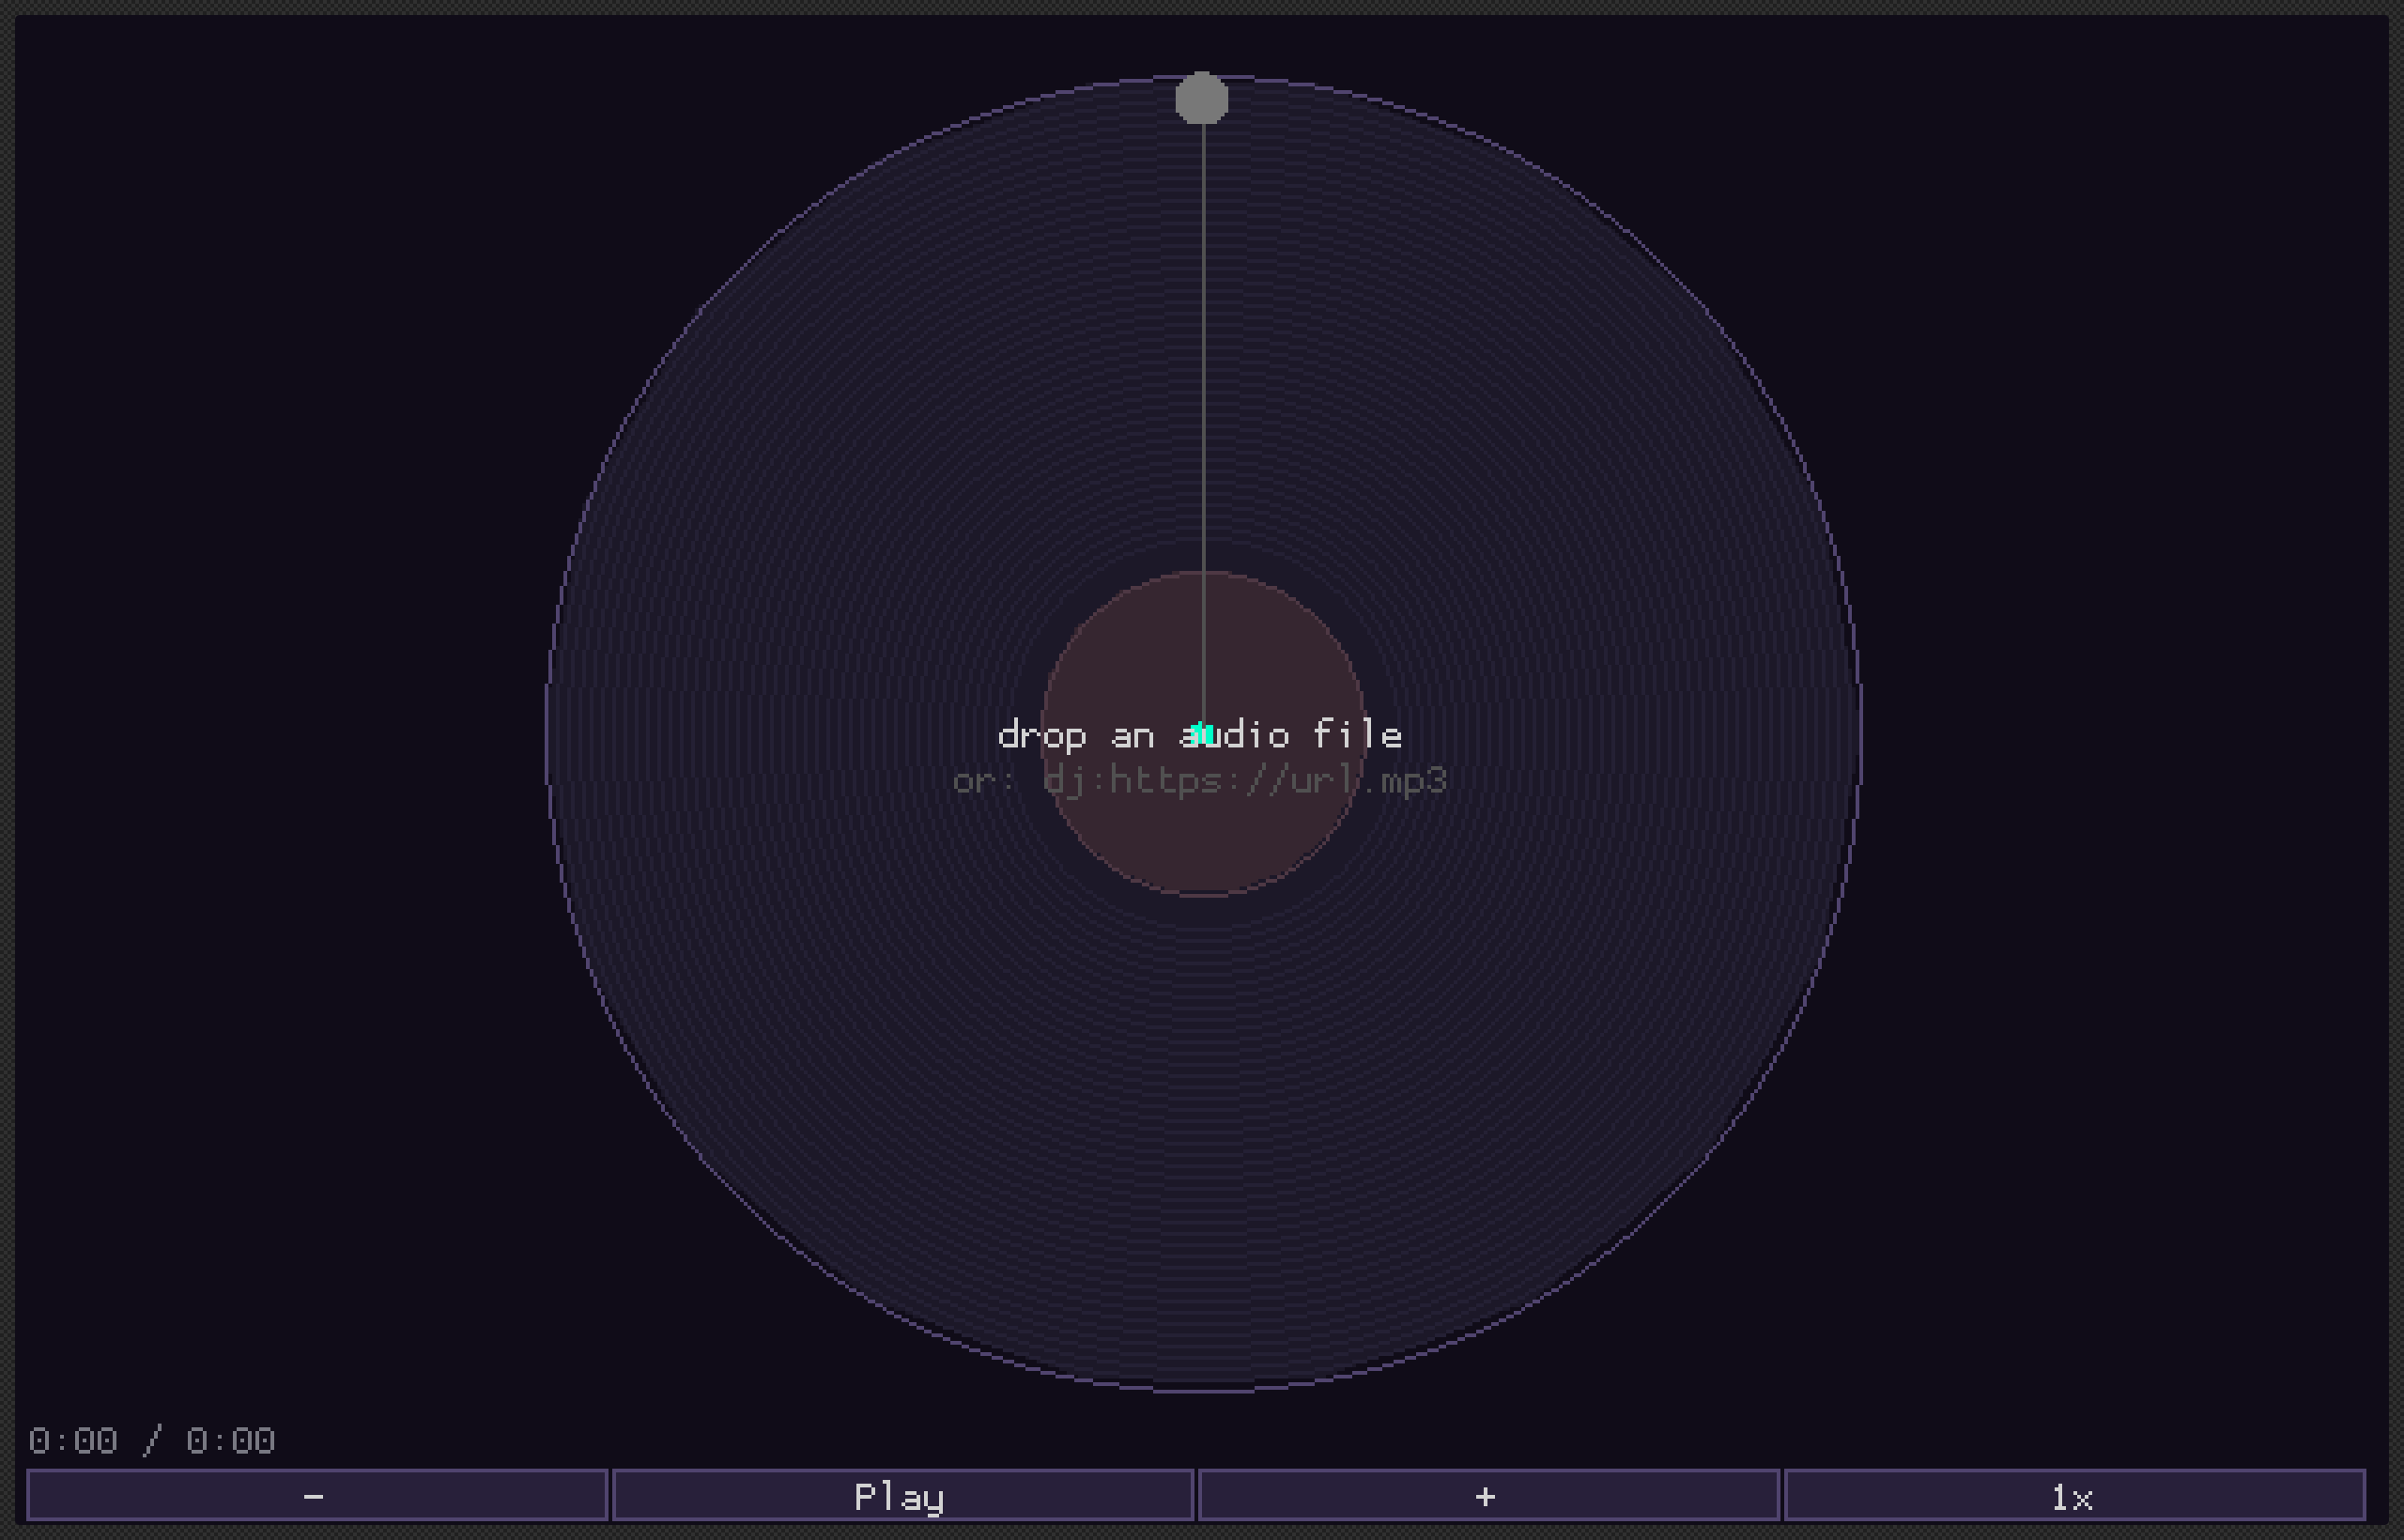
\includegraphics[width=\columnwidth]{figures/fig-ac-dj}
\caption{The \ac{} \texttt{dj} piece --- a scratchable record on a screen that has no record on it. The grooved platter turns under a tonearm and needle; dragging it radially bends pitch and rate in real time, and the label waits for a track (\texttt{drop an audio file / or: dj:https://url.mp3}). The transport strip at the bottom ($-$, \textsc{play}, $+$, $1{\times}$) is the fallback --- but it is the record, not the readout, that you play.}
\label{fig:acdj}
\end{figure} The gesture is radial: the interface takes the angular change of your pointer around the center of the platter and turns it into a signed rate --- twist the record forward and it plays forward with the pitch riding up, wind it back and it reverses. There is a pitch fader, and a waveform strip you can needle-drop into. This is the turntablist's mapping from \S4 --- position to phase, velocity to rate and pitch --- rebuilt as a piece you can open by typing a word.

I will be honest about the seam, because the two versions differ. In the browser, the audio backend cannot truly run in reverse, so forward drags are audibly pitch-bent while backward drags scrub by seeking silently --- vinyl-ish, within the limits of a web audio element, and the code says so in its own comments. The \ac{} native build has no such limit: it scratches a bespoke C audio deck that runs genuinely bidirectionally, clamped to $\pm4\times$, mixing a fractional ring-buffer read with interpolation so reverse playback is real sound, not a silent seek. So the web \texttt{dj} is an honest approximation and the native one is the real thing --- but both put a scratchable record on a screen that has no record on it.

\subsection{Why it was even possible}

None of this required special hardware. It falls out of one decision in the input layer: pieces receive continuous pointer data --- position, and a per-frame \emph{delta} that is effectively velocity (\texttt{lib/pen.mjs}). The tape scrubber and the turntable both read that same delta stream and turn it into rate. Buxton's continuous degrees of freedom (\S2) are just \emph{there}, handed to every piece, so building an instrument out of them is the path of least resistance rather than a special effort. That is the whole trick: if your platform gives pieces raw continuous gesture instead of pre-chewed widget events, the expressive playback surface is easier to build than the menu.

\subsection{Where it stops}

Being honest about the edges matters more than the pitch. Two things are not there yet. Generative time in KidLisp~\citep{scudder2026kidlisp} is monotonic and clock-synced --- you cannot yet grab a running generative piece and scrub its computation backward; the only "timeline" in the language is note scheduling. And the standalone tape \emph{replay} surface still lists play/pause and frame-by-frame scrubbing as an open to-do; today it auto-plays. Pointer \emph{pressure} is plumbed through the input layer but effectively disabled on most paths, so I am not claiming pressure-driven playback as shipped. What is real is the part that matters for the argument: continuous, gestural, real-time, pitch-coupled control of recorded audio and video, on a phone, as the default --- the exact thing the consumer platforms decided you get a dropdown for instead.

\section{The Gap Is a Market}

Line up the three claims. The coarse menu is a real, diagnosable design failure, not a sensible simplification (\S2). Fine, expressive, real-time playback control is a mature, commoditized craft, not an unsolved research problem (\S4). And a working example runs on a phone, on by default (\S5). That adds up to a specific opening --- but I have to name it precisely, because the naive version of the claim is false and a reviewer would be right to say so.

Here is the false version: \emph{nobody offers this}. They do. HCI research shipped continuous, gestural, bidirectional audio scrubbing --- pitch-preserving stretch, the sound as its own feedback --- two decades ago: Lee and Borchers' \emph{DiMaß} did in 2006 almost exactly what \S5's tape player does now~\citep{lee2006dimass}, and Beaudouin-Lafon had already named the underlying move, \emph{instrumental interaction} --- the interface as an instrument acting on the object, not a proxy describing changes to it~\citep{beaudouinlafon2000instrumental}. Consumers have had the instrument too. \emph{djay} puts a scratchable turntable over Apple Music, Spotify, and TIDAL and has passed seventy million downloads~\citep{algoriddim2024djay}; a whole mobile-DJ category sits beside it; \emph{Anytune} serves the continuous, pitch-decoupled, fine-tempo listening niche as a practice tool~\citep{anytune2024}. A dominant platform has even patented the metaphor: Google's gesture-driven video scrubbing is described, in the patent itself, as ``a disc jockey scratching records''~\citep{google2019scrubbingvideo}. The instrument is neither new nor unbuilt.

So here is the claim that actually survives, and it is sharper than the one it replaces. The instrument exists everywhere except the one place most listening and watching happens: the default transport bar of the surfaces you passively consume through. It is always walled off into a \emph{separate} app --- a DJ tool, a practice tool --- that you leave your feed to open, never offered as the way you touch the recording you came to hear. And when someone tried to bring it inside, the incumbent shut the door: \emph{Pacemaker} shipped native, Spotify-integrated mixing to a mainstream audience, and Spotify revoked the DJ API that made it possible~\citep{pacemaker2018}. That is not a market being served. It is the exact structural refusal this paper is about, caught in the act.

That refusal is the shape of the opening. The enabling technology --- pitch-preserving stretch, low-latency audio, continuous multi-touch input --- is a commodity available to anyone. The demand is visibly unmet even in its crudest form: for years, one of the most-requested items on Spotify's own forums has been \emph{any} speed control for music, and the answer has stayed no (Figure~\ref{fig:spotify})~\citep{spotify2026speed}.

\begin{figure*}[t]
\centering
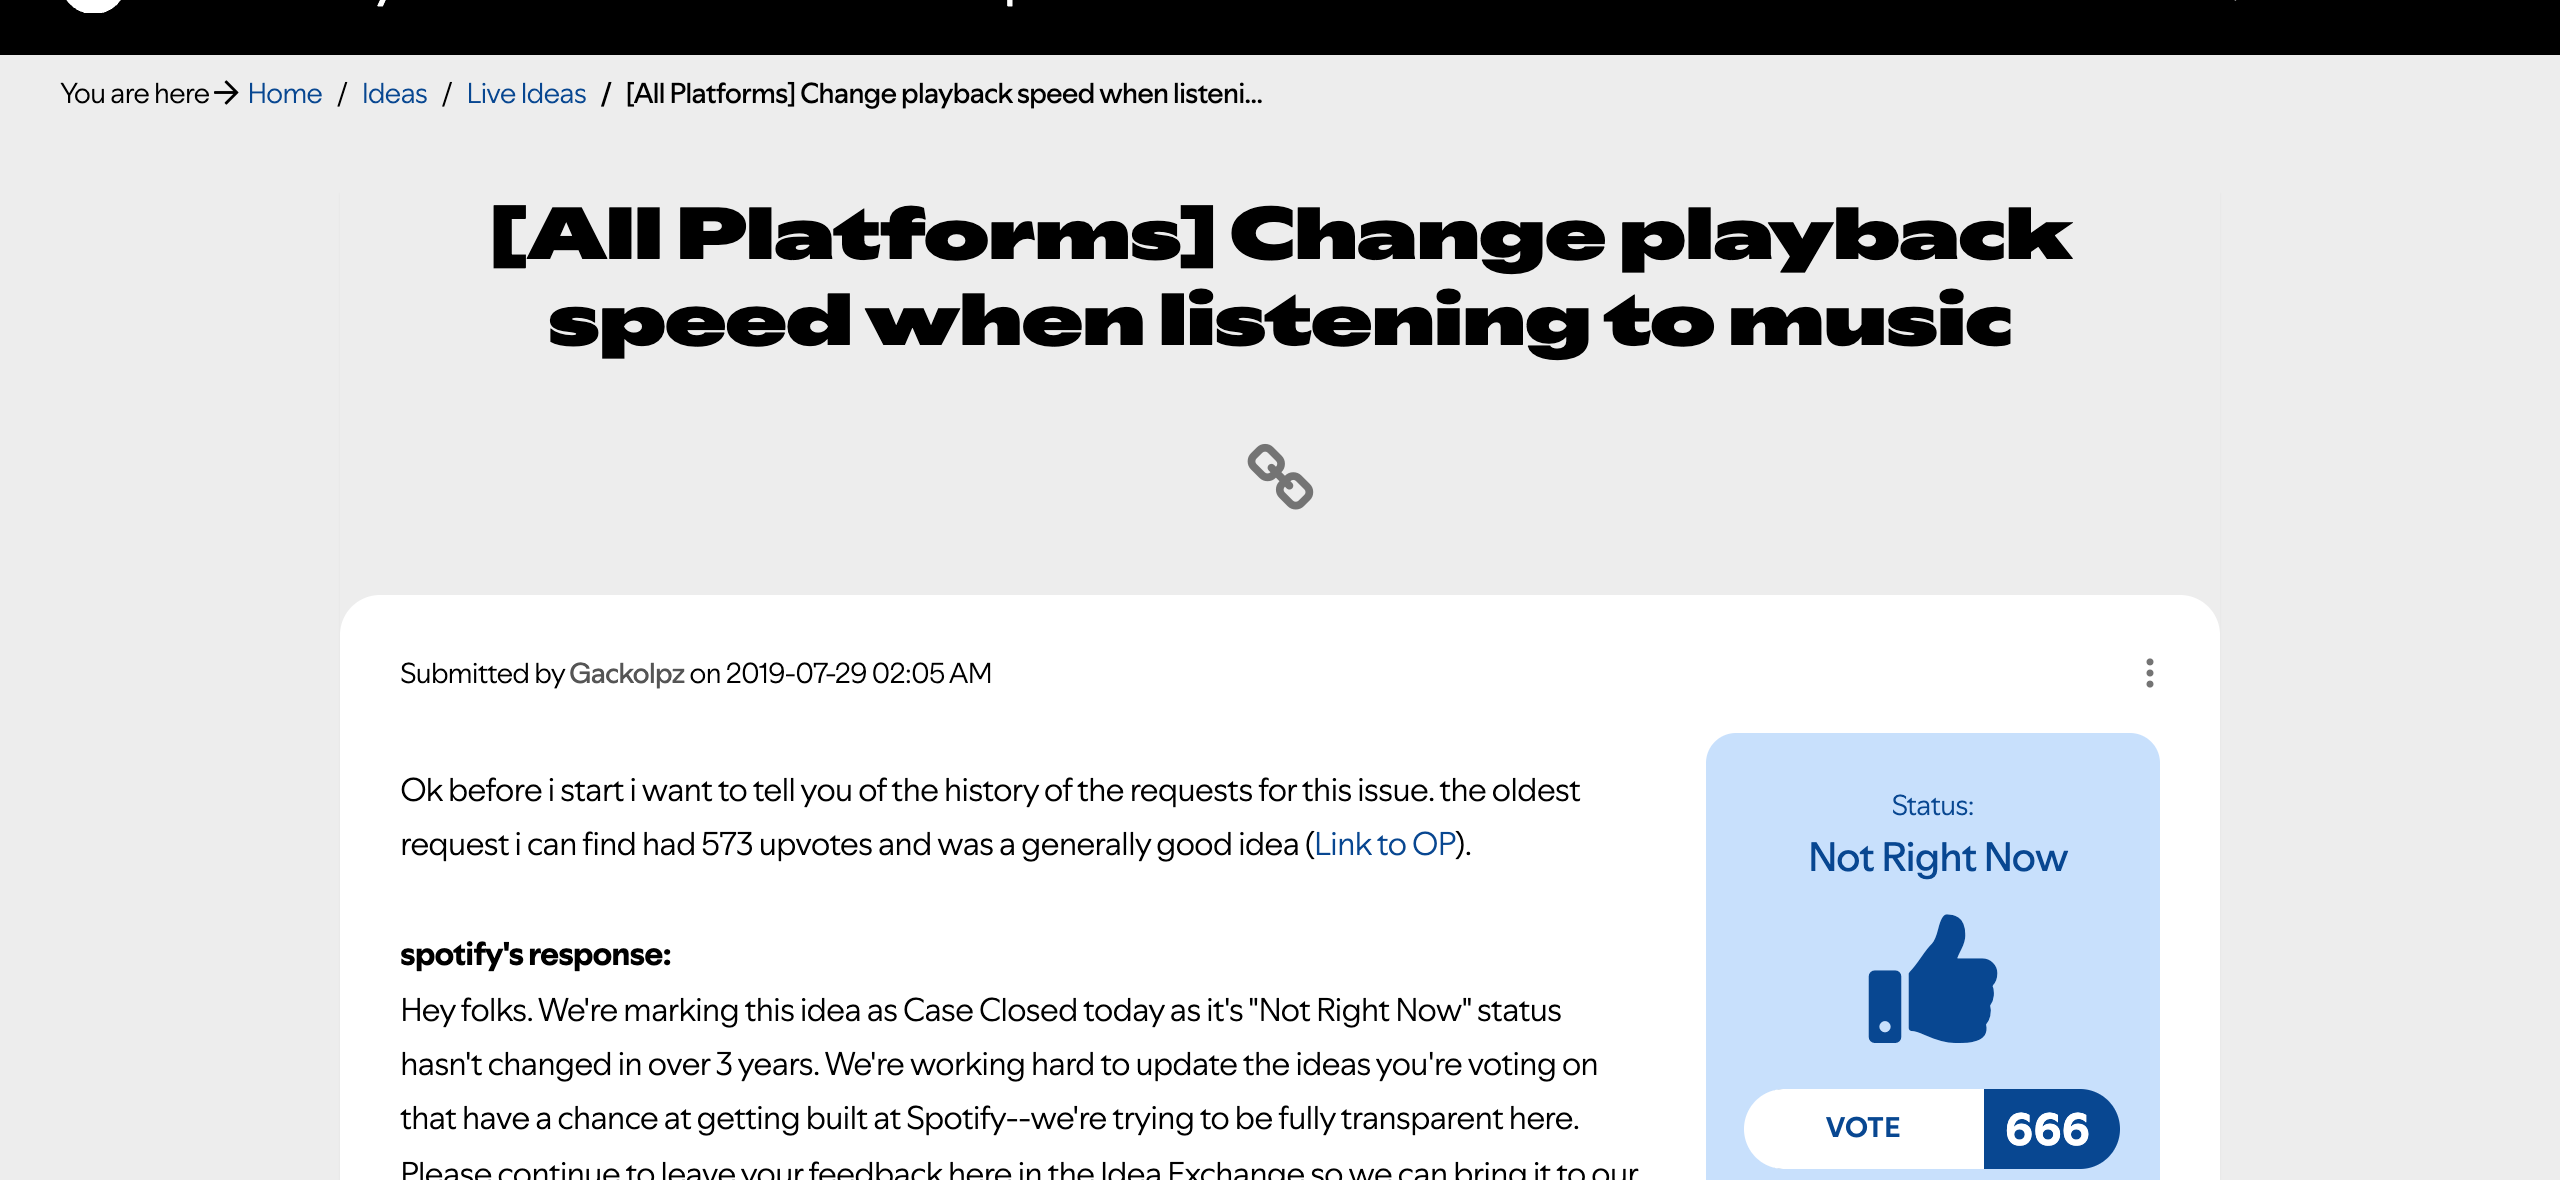
\includegraphics[width=0.88\textwidth]{figures/fig-spotify-demand}
\caption{Demand and refusal in one frame, from Spotify's own Idea Exchange. The request is only for the \emph{crude} version --- \emph{any} speed control for music --- and it has 666 votes, citing an older thread with 573. Its status is ``Not Right Now,'' and Spotify's response marks the idea \emph{Case Closed} because that status ``hasn't changed in over 3 years.'' Whatever the actual reason --- catalog licensing, artist relations, or plain deprioritization; the platform does not say --- the answer is not ``impossible.'' It is ``no.'' This is the structural refusal the paper is about, in the incumbent's own words.}
\label{fig:spotify}
\end{figure*} People are asking for a worse version of the thing this paper describes and cannot get even that. The first \emph{default transport} to treat playback as an instrument --- continuous, gestural, felt, with the media as its own feedback --- would not be competing on a feature. It would be offering a different relationship to recorded sound and image than the incumbents, locked by catalog licensing and a decade of frozen UI, have been willing to build.

\section{Limitations}

Two honest catches. First, the coarse menu is not coarse by pure stupidity --- discreteness buys real things. A five-item list is legible, thumb-reachable, accessible to a screen reader, and impossible to set to a nonsense value; a raw continuous gesture is none of those by default. Whose needs a default is built around --- the screen-reader user as much as the turntablist --- is a design-justice question, not an afterthought~\citep{costanza2020design}. The claim here is not that granularity should replace the menu but that the menu should stop being the ceiling: an expressive gestural layer can sit \emph{over} a discrete fallback, the way a DJ controller has both a jog wheel and a tempo readout. Any real product has to design that coexistence, and this paper does not.

Second, the case that expression is \emph{wanted in the default transport} at consumer scale is made here by possibility and adjacency, not by a controlled study. Turntablists want it; producers want it; \emph{djay}'s seventy million downloads and the Spotify forum threads want at least a crude version of it. But wanting a separate DJ app, or a faster podcast, is not proof that a general audience reaches for gestural rate control when it is simply \emph{there} in the player they already use --- the way it once had to be shown that they would reach for pinch-to-zoom. That is an empirical question, and the honest answer is that we will know when someone ships it well in the default. AC is where I am testing it, but AC's audience is self-selected toward exactly the people most likely to say yes.

\section{Conclusion}

The record scratch is the counterexample that should embarrass the whole consumer playback industry. It is old, cheap, physical, and expressive, and a fifteen-year-old can do things with it that a billion-dollar streaming app forbids its paying subscribers. Somewhere between the turntable and the phone, the recording stopped being something you touch and became something you configure --- and the interface that did that, the itemized speed menu, is not a neutral simplification. It is the low-water mark of directness, and we have been standing on it so long we mistook it for the ground.

It is not the ground. Fine, gestural, real-time control of recorded media is solved, mature, and portable --- researchers built it in 2006, DJ apps ship it to millions, and \ac{} already runs it across its players because I could not see a reason not to. The instrument exists. What is still empty is the one place it would matter most: the default transport bar of the surfaces you actually listen and watch through, where the incumbents --- for reasons of catalog licensing and frozen UI, not of possibility --- keep handing you a menu instead. Playback wants to be played. Somebody is going to put the instrument where the listening happens, and the gap between the scratch and the dropdown is exactly how much room there is to do it.

\vspace{1em}
{\footnotesize\color{acgray}\noindent\textit{Colophon.} Built from commit \texttt{\paperhash}, revision~\paperrev, with \mbox{Xe\TeX} on the Latin Modern / YWFT Processing type system. Working draft --- not for citation.\par\paperhistory}

\bibliographystyle{plainnat}
\bibliography{references}

\end{document}
